
\section{Experiments}
\label{sec:experiments}

\begin{figure*}[t]
    \centering
    \begin{minipage}[t]{0.38\textwidth}
        \centering
        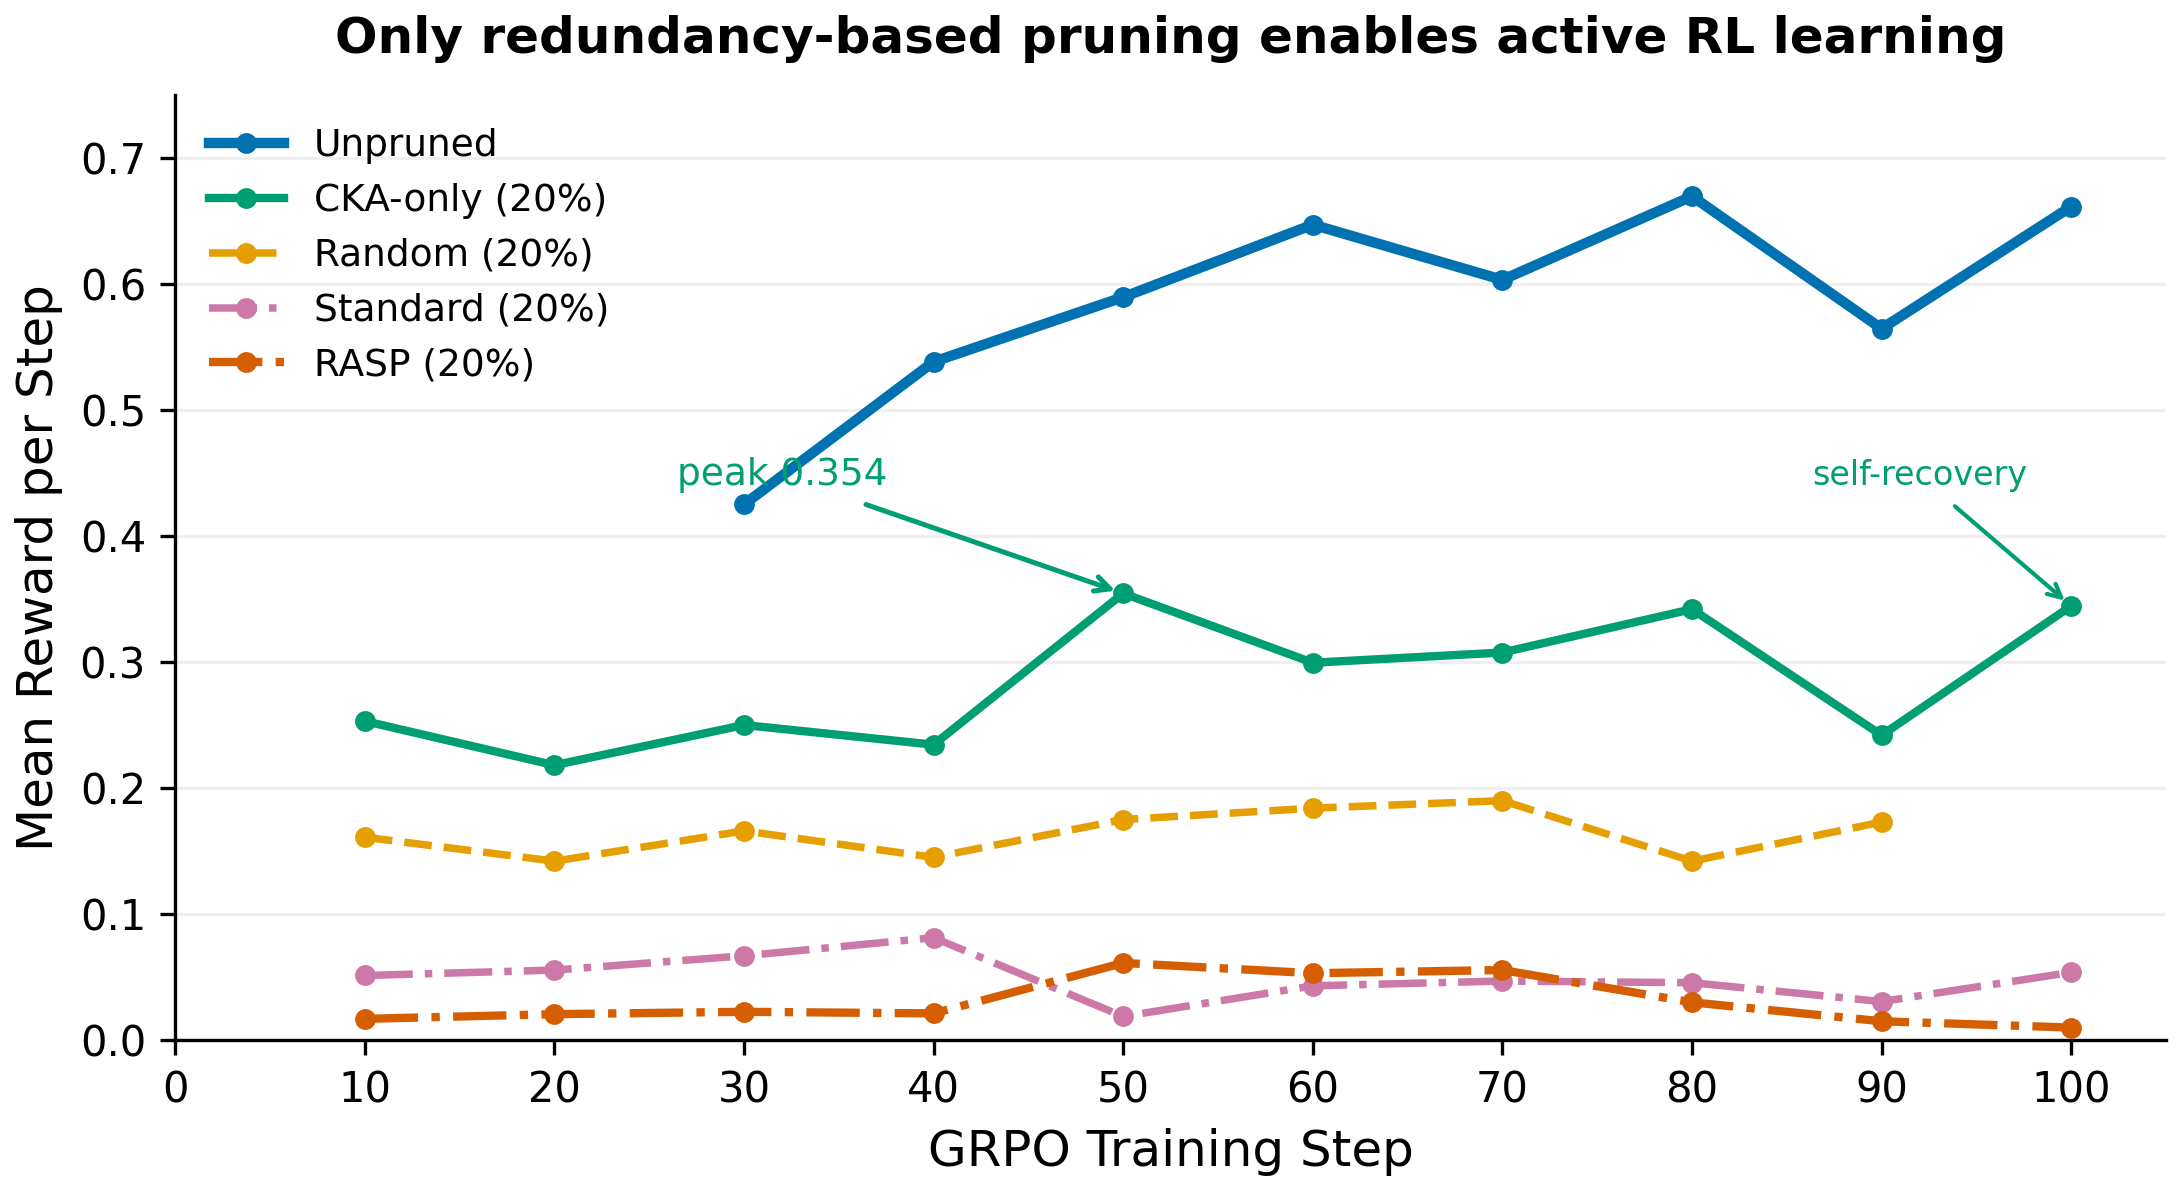
\includegraphics[width=\textwidth]{figures/paper/fig2_reward_trajectories.pdf}
        \centerline{\small (a) Reward trajectories}
    \end{minipage}
    \hfill
    \begin{minipage}[t]{0.58\textwidth}
        \centering
        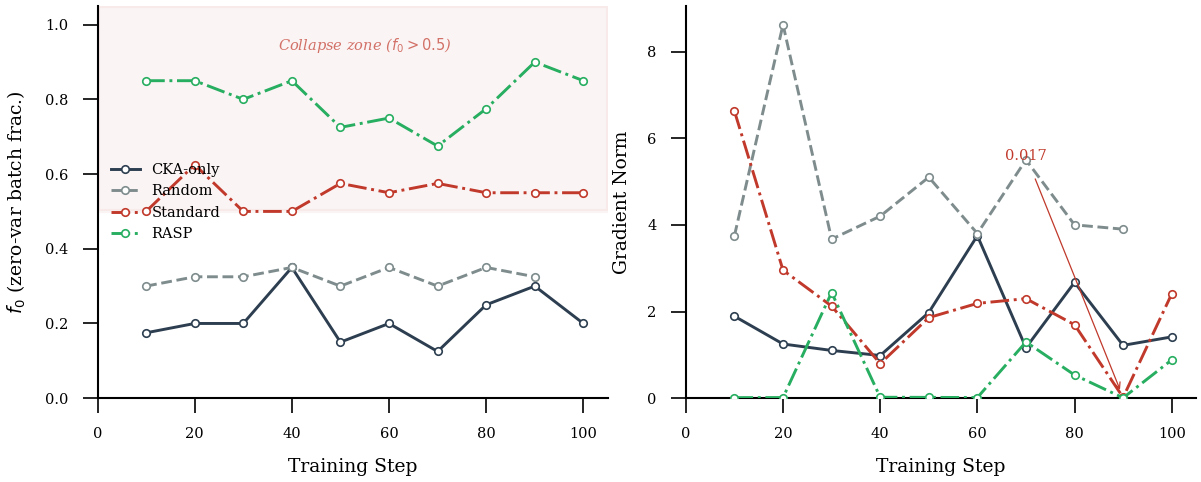
\includegraphics[width=\textwidth]{figures/paper/fig3_collapse_dynamics.pdf}
        \centerline{\small (b) $f_0$ and gradient norm diagnostics}
    \end{minipage}
    \caption{GRPO training dynamics at 20\% sparsity. (a)~Reward trajectories. (b)~$f_0$ (zero-variance batch fraction) and gradient norm diagnostics.}
    \label{fig:training_dynamics}
\end{figure*}

\subsection{Experimental Setup}
\label{sec:exp_setup}

\begin{table}[t]
\centering
\small
\caption{Recovery capacity spectrum at 20\% sparsity. $f_0$: zero-variance batch fraction. CKA-only sustains active learning; Random stagnates; Standard shows borderline collapse; \rasp{} exhibits full collapse. Best in \textbf{bold}.}
\label{tab:recovery_gradient}
\setlength{\tabcolsep}{5pt}
\begin{tabular}{@{}lccc@{}}
\toprule
Method & Peak Rew.\,$\uparrow$ & Mean Rew.\,$\uparrow$ & Min $f_0$\,$\downarrow$ \\
\midrule
CKA-only & \textbf{0.354} & \textbf{0.285} & \textbf{0.125} \\
Random & 0.190 & 0.164 & 0.300 \\
Standard & 0.081 & 0.050 & 0.500 \\
\rasp{} ($\alpha{=}1.0$) & 0.061 & 0.031 & 0.675 \\
\bottomrule
\end{tabular}
\end{table}


\paragraph{Base model and evaluation.}
We evaluate on DeepSeek-R1-Distill-Qwen-7B~\citep{deepseek2025r1}, a 7B-parameter reasoning model built on the Qwen2.5 architecture~\citep{qwen2.5} with GQA~\citep{ainslie2023gqa} (Section~\ref{sec:prelim}).
Our primary benchmark is GSM8K~\citep{cobbe2021gsm8k} ($N{=}1{,}319$ grade-school math problems; exact-match accuracy).
The unpruned model achieves 90.83\% (greedy decoding).

\paragraph{Pruning methods.}
We compare four pruning criteria at 20\% structured sparsity, all removing 200 of 784 MLP channel groups across 28 layers (${\sim}$1.45B parameters) with identical per-layer capacity floors (${\ge}$40\% retention): \textbf{CKA-only} (Eq.~\ref{eq:cka_only}), \textbf{Standard} (Eq.~\ref{eq:standard}; LLM-Pruner~\citep{llmpruner2023}), \textbf{\rasp{}} at $\alpha{=}1.0$ (Eq.~\ref{eq:score}), and \textbf{Random} (uniform selection; uses TRL's default 512-token generation limit vs.\ 1{,}024 for other methods).
See Section~\ref{sec:scoring} and Figure~\ref{fig:pruning_decisions} for scoring details.

\paragraph{Recovery pipeline and hardware.}
Immediately after pruning, all four methods produce near-zero GSM8K accuracy ($<$2\%).
All methods undergo matched two-stage recovery (Section~\ref{sec:recovery}): SFT warmup (2 epochs, 7{,}473 GSM8K examples, 37 min) followed by GRPO (lr $1{\times}10^{-6}$, $\beta{=}0.01$, $T{=}0.4$, 100 steps on 1{,}000 problems; full hyperparameters in Table~\ref{tab:hyperparams}, Appendix~\ref{sec:appendix_training}).
We repeat GRPO with 3 seeds for CKA-only, Standard, and Random (\rasp{} at $\alpha{=}1.0$ uses a single seed); CKA-only achieves 64.39\% $\pm$ 0.19\,pp, Standard 59.84\% $\pm$ 0.38\,pp (Welch's $t$, $p{<}0.001$; Appendix~\ref{sec:appendix_seed}).
The ``Unpruned'' baseline in Table~\ref{tab:decoupling} uses the same SFT-warmup checkpoint; the 9.56\,pp gap from the pre-warmup 90.83\% reflects warmup on a reduced training set, not pruning loss.
All experiments run on 2$\times$ NVIDIA RTX PRO 6000 GPUs (94\,GB VRAM each).


\subsection{Recovery Capacity Spectrum}
\label{sec:recovery_gradient}

Under GRPO training, the four pruning criteria produce a clear recovery capacity spectrum: CKA-only $\gg$ Random $\gg$ Standard $>$ \rasp{} at $\alpha{=}1.0$ (Table~\ref{tab:recovery_gradient}, Figure~\ref{fig:training_dynamics}).
The pruning criterion, rather than training configuration, determines whether the model learns, stagnates, or collapses.

Among these configurations, only the diversity-maximizing criterion (CKA-only) sustains active learning: peak reward 0.354 with $f_0$ as low as 0.125 (Figure~\ref{fig:training_dynamics}b).
Random, under a shorter generation limit, stagnates (reward 0.14--0.19, min $f_0 = 0.300$); Standard exhibits borderline collapse ($f_0 \geq 0.50$, peak reward 0.081); \rasp{} at $\alpha{=}1.0$ exhibits complete reward collapse ($f_0 \geq 0.675$, reward declining to 0.010, with near-zero KL divergence consistent with minimal policy movement; Appendix~\ref{sec:appendix_kl}).

This ordering does not mirror post-SFT accuracy.
\label{sec:sft_gradient}
Under SFT alone the ranking is CKA-only $>$ \rasp{} at $\alpha{=}1.0$ $>$ Standard $>$ Random, yet the spectrum reverses the \rasp{}/Standard ordering: Standard exhibits higher peak reward than \rasp{} despite lower SFT accuracy (Table~\ref{tab:recovery_gradient}).
The spectrum thus tracks structural properties rather than training-stage accuracy, and the dose-response analysis (\S\ref{sec:sparsity_cliff}) confirms CKA weighting as the critical variable.
Given the scale of these dynamics, one would expect equally large accuracy differences.


\subsection{Reward-Accuracy Decoupling}
\label{sec:decoupling}

\begin{table}[t]
\centering
\small
\caption{Reward-accuracy decoupling on GSM8K ($N{=}1{,}319$, greedy decoding) at step 100. All pruned models at 20\% sparsity. Multi-seed (mean $\pm$ std) where available. Best in \textbf{bold}.}
\label{tab:decoupling}
\setlength{\tabcolsep}{4pt}
\begin{tabular}{@{}lcccc@{}}
\toprule
Method & SFT\,(\%) & GRPO\,(\%) & $\Delta$\,(pp) & Peak Rew. \\
\midrule
Unpruned & \textbf{81.27} & \textbf{81.27} & $\phantom{-}$0.00 & \textbf{0.669} \\
CKA-only & 63.91 & 64.39{\scriptsize$\pm$0.19} & $+$0.48 & 0.354 \\
Standard & 59.29 & 59.84{\scriptsize$\pm$0.38} & $+$0.55 & 0.081 \\
\rasp{} ($\alpha{=}1.0$) & 61.49 & 60.88 & $-$0.61 & 0.061 \\
Random & 51.25 & 50.72{\scriptsize$\pm$0.15} & $-$0.53 & 0.190 \\
\midrule
ShortGPT & 44.73 & 43.37 & $-$1.36 & -- \\
\bottomrule
\end{tabular}
\end{table}


\begin{figure}[t]
    \centering
    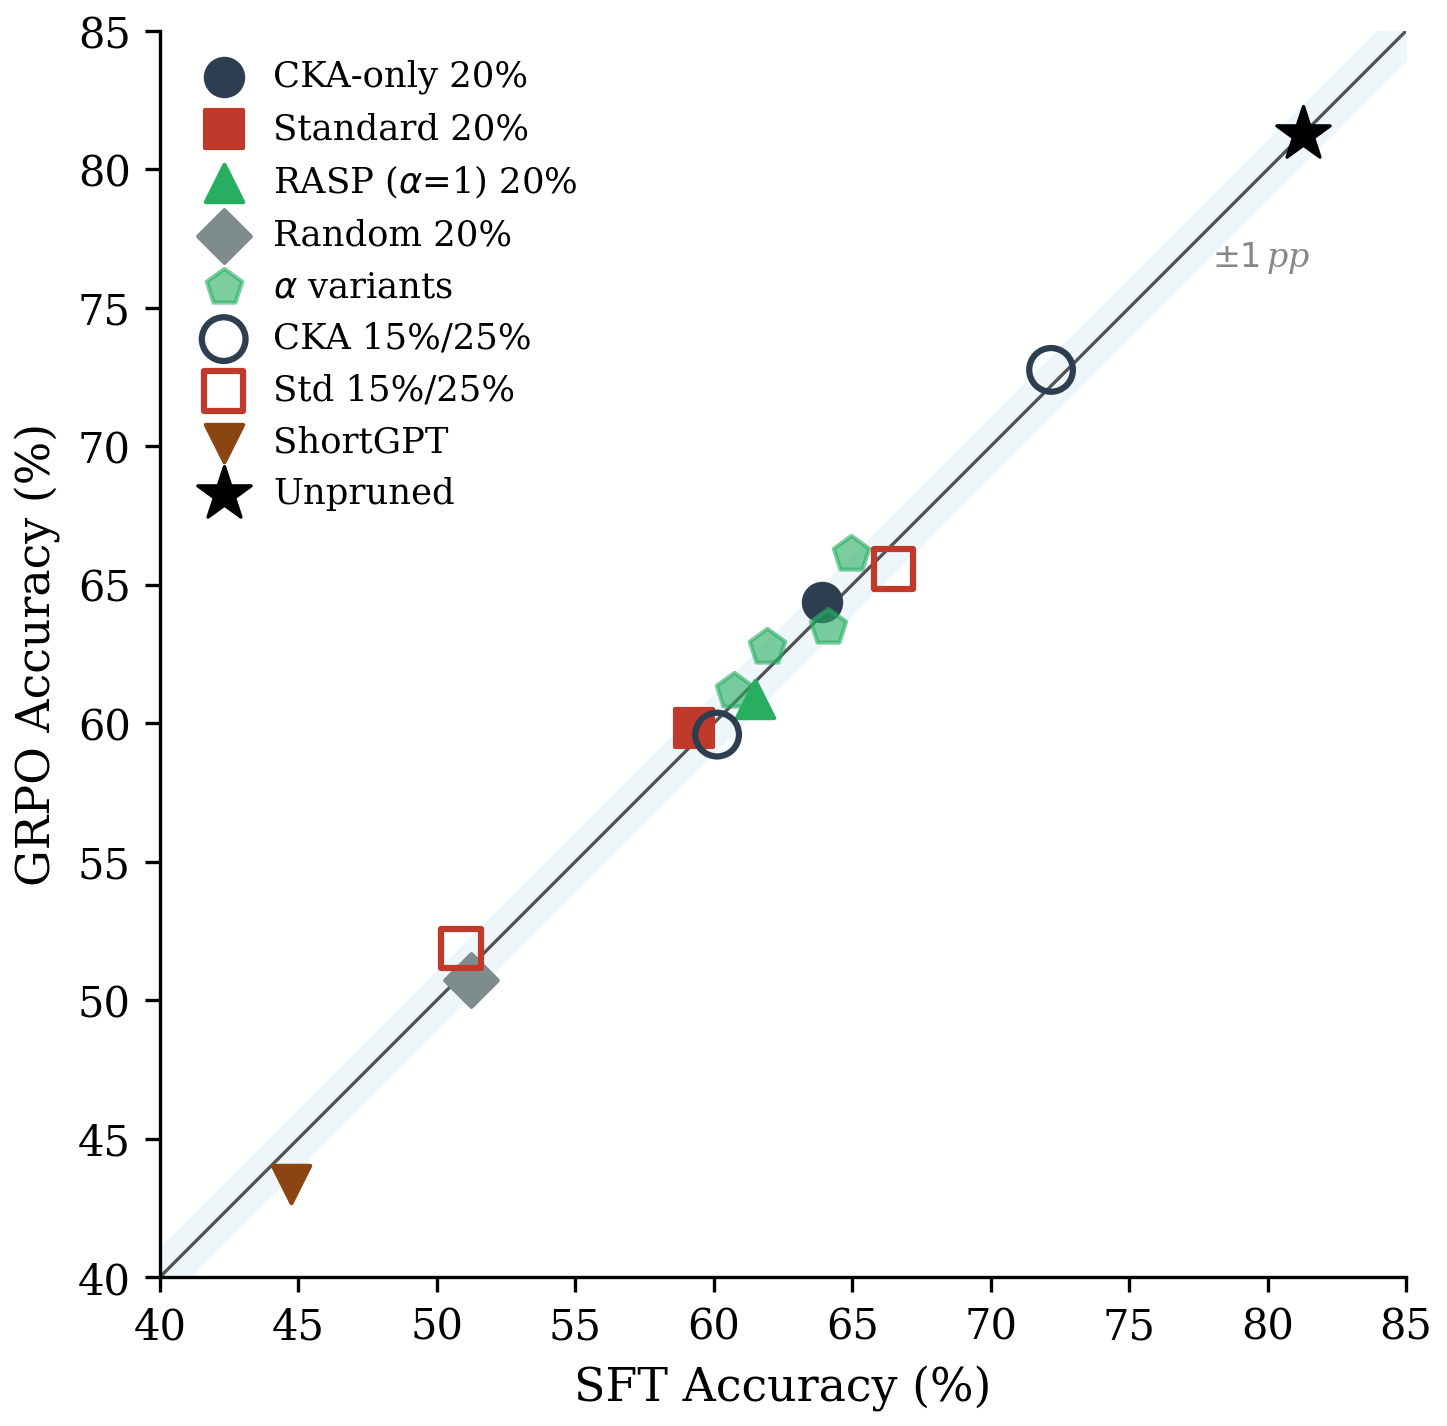
\includegraphics[width=\columnwidth]{figures/paper/fig_sft_grpo_scatter.pdf}
    \caption{SFT vs.\ GRPO accuracy on GSM8K across criteria and sparsity levels. Points near $y{=}x$ indicate reward-accuracy decoupling.}
    \label{fig:sft_grpo_scatter}
\end{figure}

The opposite holds.
Despite the 4.4$\times$ peak reward gap, GRPO produces minimal accuracy change over SFT (Figure~\ref{fig:sft_grpo_scatter}): at 20\% sparsity, all fine-grained methods differ by $|\Delta| < 1$\,pp (CKA-only $+$0.48, Standard $+$0.55, Random $-$0.53, \rasp{} at $\alpha{=}1.0$ $-$0.61\,pp; Table~\ref{tab:decoupling}).
We term this \emph{reward-accuracy decoupling} (observed at 20--25\% fine-grained MLP sparsity): reward trajectory reflects the model's capacity to learn from RL signal, not downstream accuracy.

Decoupling is not universal: at 15\% sparsity, GRPO amplifies the CKA-only advantage (SFT gap 5.69\,pp $\to$ GRPO gap 7.20\,pp), but at 20--25\% $|\Delta|$ remains below 1\,pp without exception (Tables~\ref{tab:decoupling},~\ref{tab:cross_sparsity}; Appendix~\ref{sec:appendix_cross_sparsity}), and dose-response $\alpha$ variations stay within $1.14$\,pp on GSM8K (Table~\ref{tab:alpha}).

Small $|\Delta|$ alone does not establish equivalence; it could reflect insufficient power. TOST ($\varepsilon{=}2$\,pp, substantially exceeding cross-seed $\sigma$ of 0.19--0.38\,pp; $N{=}1{,}319$ paired examples) confirm statistical equivalence for 7/8 comparisons ($p{<}0.05$; Appendix~\ref{sec:appendix_tost}), robust across seeds (0.37\,pp range; Appendix~\ref{sec:appendix_multiseed}) and extended training (300 steps; \S\ref{sec:extended_analysis}).
Directional trends hold on MATH-500~\citep{hendrycks2021math} (CKA-only and Standard rank above \rasp{} and Random; gap compression at higher difficulty; Appendix~\ref{sec:appendix_math500}) and MBPP~\citep{austin2021mbpp} (all fine-grained GRPO $|\Delta| < 2$\,pp; Appendix~\ref{sec:appendix_mbpp}).
\label{sec:ood}
ShortGPT~\citep{shortgpt2024} depth pruning is the sole exception: its GRPO delta is task-dependent ($-$1.36\,pp on GSM8K, $+$4.01\,pp on MBPP; Tables~\ref{tab:decoupling},~\ref{tab:mbpp}), unlike fine-grained methods ($|\Delta| \leq 1.8$\,pp), which suggests that layer-level removal interacts differently with RL recovery.


\subsection{Dose-Response Analysis}
\label{sec:additional_results}

\label{sec:sparsity_cliff}
The recovery capacity spectrum and decoupling raise a natural question: what controls the balance between RL trainability and final accuracy?
The CKA coefficient $\alpha$ provides a continuous knob.
On GSM8K, recovery follows an inverted-U across $\alpha \in \{0.5, 1.0, 2.0, 3.0, 4.0\}$, peaking at $\alpha{=}2.0$ (66.11\%; Figure~\ref{fig:dose_response}, Table~\ref{tab:alpha}) with $|\Delta| \leq 1.14$\,pp; \rasp{} at $\alpha{=}1.0$ exhibits reward collapse while \rasp{} at $\alpha{=}4.0$ recovers to 62.77\% (Appendix~\ref{sec:appendix_alpha}).
The pattern generalizes to MATH-500 ($\alpha{=}1.0$ worst at 23.0\%; higher-$\alpha$ cluster at 27.2--27.6\%; Table~\ref{tab:math500}).
All methods collapse at 30\% sparsity (Appendix~\ref{sec:appendix_sparsity_cliff}); pruning reduces parameters by 19\% and memory by ${\sim}$28\% (Appendix~\ref{sec:appendix_inference}).


\subsection{Structural Evidence}
\label{sec:extended_analysis}

\begin{figure*}[t]
\begin{minipage}[t]{0.48\textwidth}
    \centering
    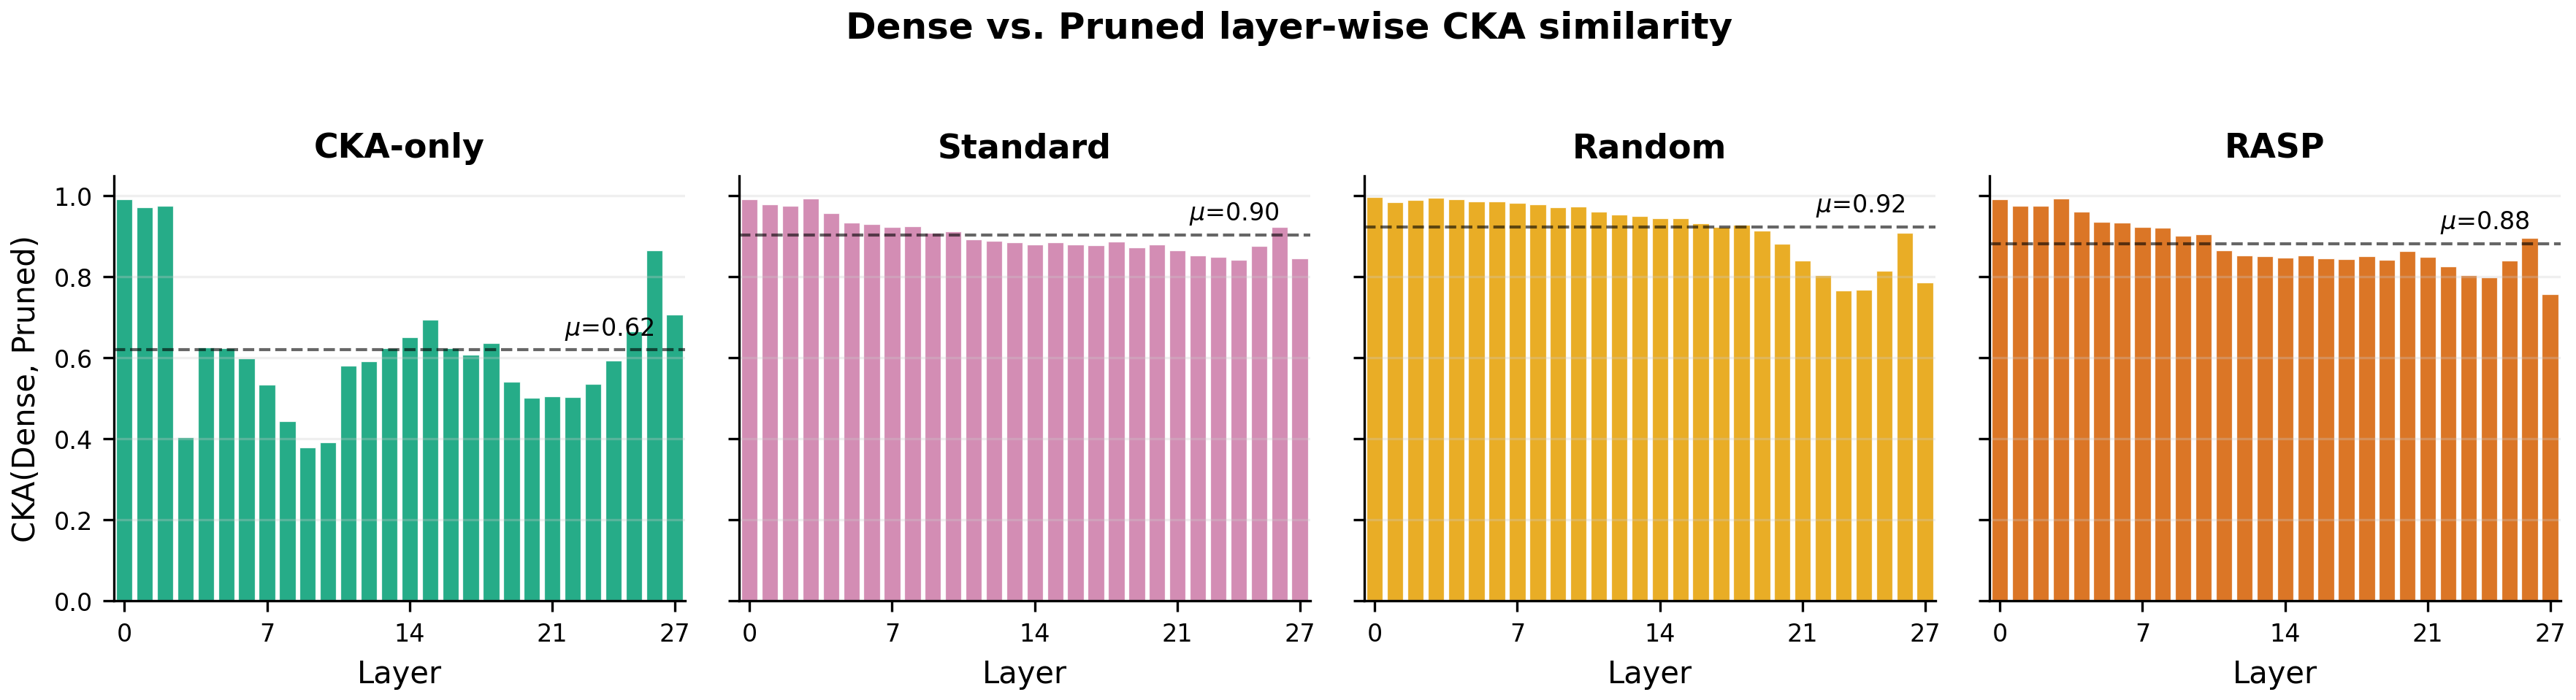
\includegraphics[width=\textwidth]{figures/paper/fig4_cka_heatmap.pdf}
    \caption{Layer-wise CKA similarity between dense and pruned representations. CKA-only diverges most ($\mu{=}0.62$) yet recovers best; importance-preserving criteria cluster near 1.0.}
    \label{fig:cka_heatmap}
\end{minipage}
\hfill
\begin{minipage}[t]{0.48\textwidth}
    \centering
    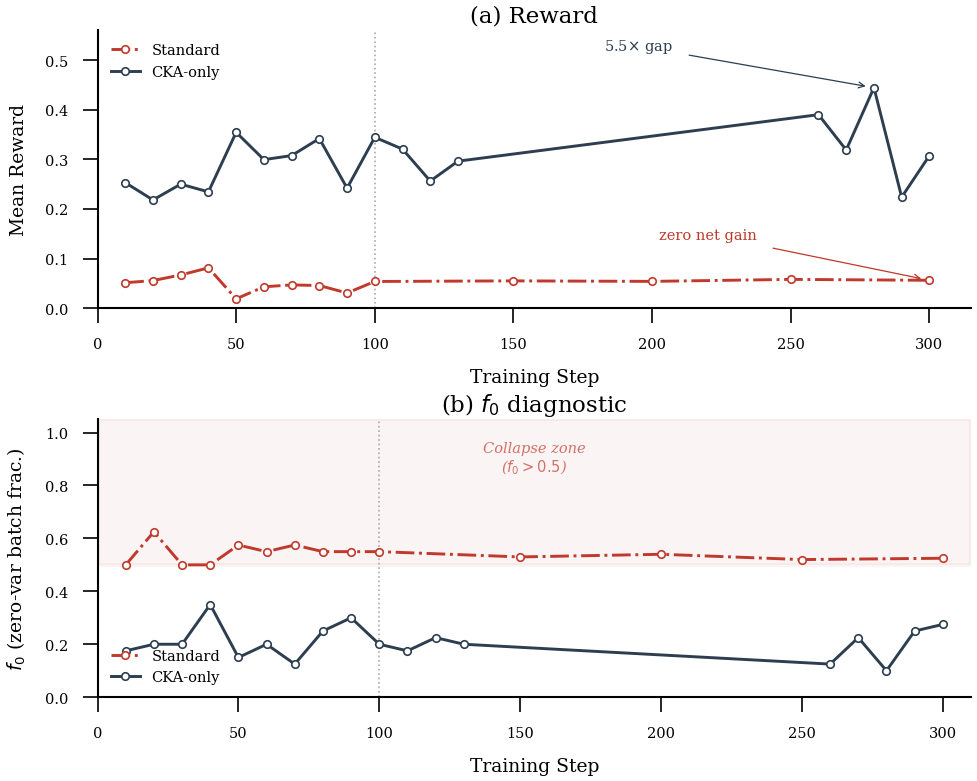
\includegraphics[width=\textwidth]{figures/paper/fig5_extended_training.pdf}
    \caption{Extended GRPO training (300 steps). (a)~Reward: Standard shows no net gain; CKA-only sustains a 5.5$\times$ gap. (b)~$f_0$: Standard remains in collapse zone.}
    \label{fig:extended_training}
\end{minipage}
\end{figure*}

\paragraph{Representational diversity.}
If diversity preservation drives recovery capacity, CKA-only should diverge most from the dense model in representation space.
Figure~\ref{fig:cka_heatmap} confirms this: CKA-only shows the lowest layer-wise CKA similarity ($\mu{=}0.62$), while Standard ($\mu{=}0.90$), Random ($\mu{=}0.92$), and \rasp{} at $\alpha{=}1.0$ ($\mu{=}0.88$) cluster near 1.0; high fidelity to the dense model comes at the cost of diversity.
One hypothesis is that removing high-overlap structures encourages redistribution of computation across diverse pathways: such structures may produce varied responses to the same prompt, providing the reward variance that GRPO requires for policy improvement.
CKA-only concentrates pruning in early layers (L0--9, 72.5\% of removed groups; Appendix~\ref{sec:appendix_overlap},~\ref{sec:appendix_depth_first}), yielding 2.89$\times$ mean gradient magnitude versus Standard (55/56 layer groups $p{<}0.05$; Appendix~\ref{sec:appendix_gradient}).
On MATH-500, CKA-only truncates only 22\% of completions (mean 655 tokens) versus Standard's 44\% (mean 1{,}128 tokens), yet achieves equal or higher accuracy (Table~\ref{tab:math500}).

\paragraph{Extended training does not resolve collapse.}
A natural objection is that importance-dominated criteria simply need more training.
When GRPO is extended from 100 to 300 steps (Figure~\ref{fig:extended_training}; Appendix~\ref{sec:appendix_extended}), Standard shows no net improvement (reward 0.054--0.058, $f_0 > 0.5$ throughout), while CKA-only sustains a 5.5$\times$ gap (0.308 vs.\ 0.056 at step 300). This persistent gap confirms that the divergence is structural rather than a matter of training budget.
The $f_0$ trajectory reinforces this conclusion: Standard enters the collapse zone ($f_0 > 0.5$) within the first 10 steps and never recovers, while CKA-only maintains $f_0 < 0.35$ throughout.
This suggests that the capacity for reward-driven learning is largely shaped at pruning time: importance-preserving pruning appears to produce a structurally homogeneous model that struggles to generate the response diversity GRPO requires, and additional training does not compensate within the horizon tested.

\paragraph{Cross-scale and cross-model generalization.}
The spectrum ordering also holds beyond the primary model.
Preliminary evidence at 1.5B scale (Table~\ref{tab:cross_scale}; Appendix~\ref{sec:appendix_cross_scale}) preserves the three-method ordering, and on Qwen2.5-Math-7B (Appendix~\ref{sec:appendix_cross_arch}), CKA-only recovers from 1.0\% post-prune to 51.50\% vs.\ Standard's 21.00\%.
This 30.5\,pp cross-model gap, substantially larger than the 4.6\,pp difference on the primary model, suggests that diversity preservation becomes increasingly important as architectural variations reduce the transferability of importance-based scoring.


